%%%%%%%%%%%%%%%%%%%%%%%%%%%%%%%%%%%%%%%%%%%%%%%%%%%%%%%%%%%%%%%%%%%%%%%%%%%%%%
% University of Bristol presentation theme based on the PowerPoint template
%
% Copyright (c) 2012, 2020 David A.W. Barton (david.barton@bristol.ac.uk)
% All rights reserved.
%
% The latest version of this theme can be found at
%   https://github.com/db9052/UoB-beamer-theme
%
% Redistribution and use in source and binary forms, with or without
% modification, are permitted provided that the following conditions are met:
%
%     * Redistributions of source code must retain the above copyright
%       notice, this list of conditions and the following disclaimer.
%     * Redistributions in binary form must reproduce the above copyright
%       notice, this list of conditions and the following disclaimer in the
%       documentation and/or other materials provided with the distribution.
%     * Neither the name of the University of Bristol nor the names of its
%       contributors may be used to endorse or promote products derived from
%       this software without specific prior written permission.
%
% THIS SOFTWARE IS PROVIDED BY THE COPYRIGHT HOLDERS AND CONTRIBUTORS "AS IS"
% AND ANY EXPRESS OR IMPLIED WARRANTIES, INCLUDING, BUT NOT LIMITED TO, THE
% IMPLIED WARRANTIES OF MERCHANTABILITY AND FITNESS FOR A PARTICULAR PURPOSE
% ARE DISCLAIMED. IN NO EVENT SHALL <COPYRIGHT HOLDER> BE LIABLE FOR ANY
% DIRECT, INDIRECT, INCIDENTAL, SPECIAL, EXEMPLARY, OR CONSEQUENTIAL DAMAGES
% (INCLUDING, BUT NOT LIMITED TO, PROCUREMENT OF SUBSTITUTE GOODS OR SERVICES;
% LOSS OF USE, DATA, OR PROFITS; OR BUSINESS INTERRUPTION) HOWEVER CAUSED AND
% ON ANY THEORY OF LIABILITY, WHETHER IN CONTRACT, STRICT LIABILITY, OR TORT
% (INCLUDING NEGLIGENCE OR OTHERWISE) ARISING IN ANY WAY OUT OF THE USE OF
% THIS SOFTWARE, EVEN IF ADVISED OF THE POSSIBILITY OF SUCH DAMAGE.
%%%%%%%%%%%%%%%%%%%%%%%%%%%%%%%%%%%%%%%%%%%%%%%%%%%%%%%%%%%%%%%%%%%%%%%%%%%%%%
\documentclass[aspectratio=169]{beamer}
    % Possible aspect ratios are 16:9, 16:10, 14:9, 5:4, 4:3 (default) and 3:2
    % (Remember to remove the colon, i.e., 16:9 becomes the option 169)

\graphicspath{ {../img/} }
\usetheme{UoB}
\usepackage{multicol,tikz}
\usepackage[vlined,linesnumbered]{algorithm2e}
\usetikzlibrary{automata,positioning,arrows.meta}
\setlength{\parskip}{.3\baselineskip}
% If lualatex is used then Rockwell, Latin Modern math, and Arial are used as
% per the UoB style. If pdflatex is used then Concrete, Euler math, and
% Helvetica are used as the closest alternatives.

%%%%%%%%%%%%%%%%%%%%%%%%%%%%%%%%%%%%%%%%%%%%%%%%%%%%%%%%%%%%%%%%%%%%%%%%%%%%%%
\title[Short Title]{Summary Statistic Selection for Approximate Bayesian Computation}
\subtitle{Can the machines do it?}
\author{Dom Hutchinson}
% \institute{Job Title or Affiliation}
\date{06/05/2021}

\AtBeginSection[]{
  \begin{frame}[leftcolor=CoolGrey,rightcolor=UniversityRed,div=0.85\paperwidth]
  \vfill
  \centering
  \begin{beamercolorbox}[sep=8pt,center,shadow=false,rounded=true]{title}
    \usebeamerfont{title}\insertsectionhead\par%
  \end{beamercolorbox}
  \vfill
  \end{frame}
}

%%%%%%%%%%%%%%%%%%%%%%%%%%%%%%%%%%%%%%%%%%%%%%%%%%%%%%%%%%%%%%%%%%%%%%%%%%%%%%
% Lectures to include

% Lectures available (see \lecture commands below):
%   01: Introductory slides

\ifdefined\uselecture
  % Automatically generate specific lecture slides: run (lua/pdf)latex with
  % latex -jobname "slides-01" "\def\uselecture{01}\input{slides.tex}"
  % latex -jobname "handout-01" "\def\uselecture{01}\PassOptionsToClass{handout}{beamer}\input{slides.tex}"
  \expandafter\includeonlylecture\expandafter{\uselecture}
\else
  % Default lecture to output - comment out to get all lectures
  \includeonlylecture{01}
\fi

% Uncomment to get title slides for each lecture
% \AtBeginLecture{
%   \subtitle{\insertlecture}
%   \setcounter{framenumber}{0}
%   \begin{frame}
%     \titlepage
%   \end{frame}
% }

%%%%%%%%%%%%%%%%%%%%%%%%%%%%%%%%%%%%%%%%%%%%%%%%%%%%%%%%%%%%%%%%%%%%%%%%%%%%%%
% Start of the slides

\begin{document}

% Available frame options:
%   leftcolor, rightcolor: set the colour of the left or right panel
%   leftimage, rightimage: put a (cropped) image in the left or right panel
%   div: set the location of the divider between left and right panels
%   urlcolor: set the colour of the url

% Other commands available:
%   \logo{X}: choose the logo to display (logo, white logo, or black logo)
%   \urltext{X}: change the url for each slide

% All standard University of Bristol colours are available:
%   UniversityRed, CoolGrey, BrightAqua, BrightBlue, BrightOrange, BrightPurple,
%   BrightPink, BrightLime, DarkAqua, DarkBlue, DarkOrange, DarkPurple,
%   DarkPink, DarkLime

\begin{frame}[leftcolor=CoolGrey,rightcolor=UniversityRed,div=0.85\paperwidth]
  \titlepage
\end{frame}

\section{Approximate Bayesian Computation}

\begin{frame}{ABC Motivation}\small
  Computational method for approximating posteriors for the parameters $\theta$ of models $X$ where the likelihood $\mathbb{P}(X|\theta)$ is intractable.
  \[ \mathbb{P}(\theta|X)=\frac{\mathbb{P}(X|\theta)\mathbb{P}(\theta)}{\mathbb{P}(X)}\propto\mathbb{P}(X|\theta)\mathbb{P}(\theta) \]

  ABC methods target sampling from the joint distribution $\pi_{ABC}(\theta,s|s_{obs})$.
  \[ \pi_{ABC}(\theta,s|s_{obs}):=K_\varepsilon(\|s-s_{obs}\|)\mathbb{P}(s|\theta)\pi_0(\theta) \]
  Since
  \[\everymath={\displaystyle}\begin{array}{rrrl}
    &\pi_{ABC}(\theta|s_{obs})&=&\int \pi_{ABC}(\theta,s|s_{obs})ds\\
    \implies&\lim_{\varepsilon\to0}\pi_{ABC}(\theta|x_{obs})&=&\lim_{\varepsilon\to0}\int K_\varepsilon(\|x-x_{obs}\|)\mathbb{P}(x|\theta)\pi_0(\theta)dx\\
    &&=&\int \delta_{x_{obs}}(x)\mathbb{P}(x|\theta)dx\cdot \pi_0(\theta)\\
    &&=&\mathbb{P}(x_{obs}|\theta)\pi_0(\theta)\propto\mathbb{P}(\theta|x_{obs})
  \end{array}\]
\end{frame}

\begin{frame}{Approximate Bayesian Computation}
  \par \textit{General ABC Schema}
  \par\textbf{Require:} Observed values $x_{obs}$; Summary statistics $s(\cdot)$; Priors $\pi_0(\cdot)$; Theorised model $f(X|\cdot)$; Acceptance Kernel $K_\varepsilon(\cdot)$; Distance Measure $\|\cdot\|$.
  \begin{enumerate}
    \item Calculate summary statistic values $s_{obs}=s(x_{obs})$.
    \item Until stopping condition reached:
    \begin{enumerate}
      \item Sample a set of parameters $\tilde\theta$.
      \item Run the theorised model with sampled parameter $\tilde{x}=f_{\tilde\theta}(X|\tilde\theta)$.
      \item Calculate summary statistic values $\tilde{s}=s(\tilde{x})$.
      \item Accepted parameters $\tilde\theta$ with probability $K_\varepsilon(\|\tilde{s}-s_{obs}\|)$.
    \end{enumerate}
    \item Return all accepted parameter sets $\hat\Theta$.
  \end{enumerate}
\end{frame}

\begin{frame}{ABC Schema}
  \begin{figure}[H]
    \centering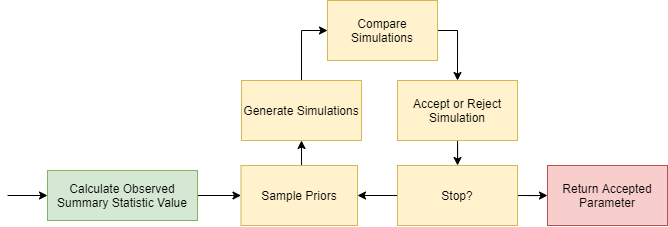
\includegraphics[width=1\textwidth]{ABC_flow.png}
    \caption{Flow-diagram for general ABC schema}
  \end{figure}
\end{frame}

\begin{frame}{ABC Algorithm Parameters}
  \setlength{\parskip}{.1\baselineskip}
  Standard ABC methods require the user to specify the following
  \begin{multicols}{2}
    \begin{itemize}
      \item Theorised Model.
      \item Priors.
      \item Summary Statistics.
      \item Acceptance Kernel.
      \item Distance Measure.
      \item Stopping Condition.
    \end{itemize}
  \end{multicols}
  \par There are several common approaches to ABC which vary how parameters are sampled, how simulations are accepted and the stopping condition:
  \begin{itemize}
    \item Rejection Sampling ABC.
    \item Markov Chain Monte Carlo ABC (ABC-MCMC) [Marjoram et al., 2003].
    \item Sequential Monte Carlo ABC (ABC-SMC). [Sisson al., 2007]
  \end{itemize}
  [Beaumontet al., 2009] discuss the most adaptive version of ABC, a variation of ABC-SMC.
\end{frame}

\section{Summary Statistics}

\begin{frame}{Summary Statistics}
  \par Large datasets take longer to process and suffer from the curse of dimensionality. For example, an SIR model over only 30 time-periods still generates 90 data-points.
  \par Summary statistics $s$ project data to lower dimensions whilst retain information.
  \[\begin{array}{rcll}
    s&:&\mathbb{R}^m\to\mathbb{R}^n&\text{ with }m>n\\
    s&:&\mathbb{R}^{m\times p}\to\mathbb{R}^n&\text{ with }m\times p>n\\
  \end{array}\]
  \par Examples: Mean, Median, Variance.
  \par In general, each dimension of the output of a summary statistic is defined independently.
  \par Summary statistics have traditionally been chosen manually using intuition and by the prevalence of the statistic in the literature.
\end{frame}

\begin{frame}{Summary Statistics - Comments}
  A good summary statistic has the following properties:
  \begin{multicols}{2}
    \begin{itemize}
      \item Minimal information loss.
      \item High dimensionality reduction.
      \item Unbiased.
      \item Computationally efficient.
      \item Map to a known dimensionality.
      \item Interpretable.
    \end{itemize}
  \end{multicols}
  In general a good fit can be achieved, for simple models, with at most one summary statistic per parameter. If parameters are highly correlated or co-linear then less summary statistics are required.
\end{frame}

\begin{frame}{Sufficient Summary Statistic}
  \par Sufficient summary statistics are those which can reduce dimensionality whilst still retain all the information contained in the full data set.
  \[ \mathbb{P}(X|s(X))=\mathbb{P}(X|s(X),\theta) \]
  \par Example: The sample mean is a sufficient statistic for a normal distribution with unknown mean, but known variance.
  \par The identity function is a sufficient statistic for all models, but this is not very helpful for computational problems.
\end{frame}

\begin{frame}{Sufficient Statistics in Practice}
  \par Identifying sufficient statistics is very difficult in practice.
  \begin{theorem}[Fisher-Neyman Factorisation Criterion]
    $s(\cdot)$ is a sufficient statistic for the model parameters $\theta$ \underline{iff} there exist non-negative functions $g(\cdot;\theta)$ and $h(\theta)$ where $h(\cdot)$ is independent of the model parameters\footnotemark\footnotetext{i.e. $h(\cdot)$ only depends on the sampled data} and
    \[ f(X;\theta)=h(X)g(s(X);\theta) \]
    This formulation shows that the distribution of the model $X$ only depends on the parameter $\theta$ through the information extracted by the statistic $s$. A consequence of the sufficiency of $s$.
  \end{theorem}
\end{frame}

\section{Summary Statistic Selection Methods}

\begin{frame}{Joyce-Marjoram - Preliminaries}
  Since identifying sufficient statistics is difficult, [Joyce and Marjoram, 2008] proposes finding a set of statistics $S'$ which are approximately sufficient to some super-set $S$.
  \par They define the score metric measures how much more information a set of statistics extracts when it is extended by one statistic.

  \begin{block}{Score $\delta_k$}
    The score of $s_k$ relative to the set $s_{1:k-1}:=\{s_1,\dots,s_{k-1}\}$ is defined as
    \[ \delta_k:=\sup_\theta\left\{\ln\mathbb{P}(s_k|s_{1:k-1})\right\}-\inf_\theta\left\{\ln\mathbb{P}(s_k|s_{1:k-1})\right\} \]
  \end{block}
\end{frame}

\begin{frame}{Joyce-Marjoram - Algorithm}
  \begin{block}{Joyce-Marjoram Algorithm}
    \begin{algorithm}[H]
      \SetKwInOut{Require}{require}
      \Require{Set of summary statistics $S$; Score threshold $\varepsilon$}
      $S'\leftarrow\emptyset$\\
      \While{true}{
        Calculate the score for each statistic in $S$ wrt $S'$\label{alg_line_calculate_score}\\
        $\delta_{max}\leftarrow\max_{s\in S}\text{Score}(s;S')$\label{alg_approximately_sufficient_subsets_max_score}\\
        $s_{max}\leftarrow\text{argmax}_{s\in S}\text{Score}(s;S')$\label{alg_approximately_sufficient_subsets_max_statistic}\\
        \lIf{$\delta_{max}>\varepsilon$}{\label{alg_approximately_sufficient_subsets_if_statement}
          $S'\leftarrow S'\cup\{s\}$
        } \lElse {
          \Return{S'}
        }
      }
    \end{algorithm}
  \end{block}
  However, the score metric is intractable. The approach proposed by Joyce \& Marjoram compares the posteriors of the proposed sets and switches if the posteriors are notably different. This does not perform well with truly random summary statistics.
\end{frame}

\begin{frame}{Minimising Entropy - Preliminaries}
  Entropy is a measure of information in a distribution, with lower values indicating more information.
  \begin{block}{Entropy}
    {\small The entropy $H(X)$ of a probability distribution $X$ is a measure of the information and uncertainty in distribution.}
    \[\everymath={\displaystyle}\begin{array}{rrcl}
      \text{Discrete}&H(X)&:=&-\sum_{x\in\mathcal{X}}\mathbb{P}(X=x)\cdot\ln\mathbb{P}(X=x)%\\
      % \text{Continuous}&H(X)&:=&-\int_{\mathcal{X}}f_X(x)\cdot\ln f_X(x)dx
    \end{array}\]
    % where $\mathcal{X}$ is the support of distribution $X$.\\
  \end{block}

  \begin{block}{$k^{th}$ Nearest Neighbour Estimator of Entropy}
    \[ \hat{H}=\ln\left(\frac{\pi^{\rho/2}}{\Gamma\left(1+\frac\rho2\right)}\right)-\frac{\Gamma'(k)}{\Gamma(k)}+\ln(n)+\frac\rho{n}\sum_{i=1}^n\ln D_{i,k} \]
    {\small where $n=|\Theta|$, $\rho$ is the number of parameters, $D_{i,k}$ is the Euclidean distance between the $i^{th}$ accepted parameter set and its $k^{th}$ nearest neighbour and $\Gamma(\cdot)$ is the gamma function.}
  \end{block}
\end{frame}

\begin{frame}{Minimising Entropy - Algorithm}
  [Nunes and Balding, 2010] propose an approach to summary statistic selection which choose whichever set of statistics minimises entropy.
  \begin{block}{Minimising Entropy Summary Statistic Selection (ME)}
    \begin{algorithm}[H]
      \SetKwInOut{Require}{require}
      \Require{Set of summary statistics $S$}
      \For{$S'\in 2^{S}$}{\label{alg_me_sss_for_loop}
        $\Theta\leftarrow$Parameter sets accepted from ABC-Rejection Sampling using $S'$\label{alg_me_rejection_sampling}\\
        $\hat{H}_{S'}\leftarrow\hat{H}(\Theta)$
      }
      $S_{ME}^*\leftarrow\text{argmin}_{S'\in 2^S}\hat{H}_{S'}$\\
      \Return{$S_{ME}^*$}
    \end{algorithm}
  \end{block}

  There are several ways to estimate entropy $\hat{H}$. [Nunes and Balding, 2010] recommend the $k^{th}$-Nearest Neighbour Estimator of Entropy with $k=4$.
\end{frame}

\begin{frame}{Two Step Minimising Entropy - Algorithm}
  \begin{block}{Two Step ME Summary Statistic Selection}
    \begin{algorithm}[H]
      \SetKwInOut{Require}{require}
      \Require{Observations from true model $x_{obs}$, Set of summary statistics $S$, Number of simulations to run $n_{run}$, Number of simulations to accept $n_{obs}$} % TODO x_{obs} is required
      $S_{ME}\leftarrow$ME($S$)\\
      $\hat{\Theta}_{ME}\leftarrow${\small Parameter sets accepted from ``Best Samples'' ABC-RS($x_{obs},S_{ME},n_{run},n_{acc}$)}\\
      Standardise $\hat\Theta_{ME}$\\
      \For{$S'\in 2^{S}$}{\label{alg_two_step_me_for_loop}
      $\Theta_{acc}\leftarrow${\small Parameter sets accepted from ``Best Samples'' ABC-RS($x_{obs},S',n_{run},n_{acc}$)\\
      Standardise $\Theta_{acc}$}\\
      $\text{MRSSE}_{S'}\leftarrow\text{MRSSE}(\Theta_{acc},\hat\Theta_{ME,i})$
      }
      $S^*\leftarrow\text{argmin}_{S'\in 2^S}MRSSE_{S'}$\\
      \Return{$S^*$}
    \end{algorithm}
  \end{block}
\end{frame}

\begin{frame}{Semi-Automatic ABC}
  \footnotesize\setlength{\parskip}{.1\baselineskip}
  [Fearnhead and Prangle, 2011] propose a method which generates its own summary statistics using linear regression.
  \begin{block}{Least-Squares Semi-Automatic ABC}
    \begin{algorithm}[H]
      % \SetKwInOut{Require}{require}
      % \Require{Observations from true model $x_{obs}$, Set of summary statistics $S$, Number of simulated parameter sets $m$, Theorised model $X$, Mapping $f(\cdot)$}
      $f_\theta\leftarrow$Posterior from pilot run of an ABC-method using $x_{obs}$ and $S$\label{alg_semi_auto_abc_ls_pilot_run}\\
      $\hat\Theta\leftarrow$ $m$ simulations from $f_\theta$\label{alg_semi_auto_abc_ls_generate_1}\\
      $X_{\hat\theta}\leftarrow$ $X\left(\hat\theta\right)$ for each $\hat\theta\in\hat\Theta$\label{alg_semi_auto_abc_ls_generate_2};  $\hat{X}\leftarrow\{X_{\hat\theta_1},\dots,X_{\hat\theta_m}\}$\\
      $F\leftarrow f(\hat{X})$; $\tilde{F}\leftarrow F$ with a preceding column of 1s\\
      \For{$i=1,\dots,\rho$}{
        $A_i\leftarrow i^{th}$ element of each set in $\hat\Theta$\\
        $(\alpha^{(i)},\pmb\beta^{(i)})\leftarrow(\tilde{F}^T\tilde{F}^{-1})\tilde{F}^TA_i$\\
        $s_i(\mathbf{x}):=\pmb\beta^{(i)}\mathbf{x}$
      }
      \Return{$\{s_1,\dots,s_\rho\}$}
    \end{algorithm}
  \end{block}
  Alternatively, Lasso regression or Canonical correlation analysis can be used. Linear regression is straightforward and has closed form solutions.
\end{frame}

\section{SIR Model}

\begin{frame}{SIR Model}
  The SIR model is a compartmental model which models the movements of individuals in a population between three compartments:

  \begin{figure}[!htb]
    \centering
    \begin{minipage}{.3\textwidth}
        \centering
        \begin{itemize}
          \item \textbf{S}usceptible.
          \item \textbf{I}nfectious.
          \item \textbf{R}emoved.
        \end{itemize}
    \end{minipage}%
    \begin{minipage}{.7\textwidth}
        \centering
        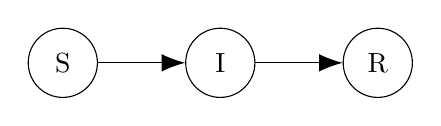
\begin{tikzpicture}[align=center,node distance=2cm and 4cm]
          \node[state] (S) {S};
          \node[state, right of=S] (I) {I};
          \node[state, right of=I] (R) {R};

          \draw (S) edge[-{Latex[length=3mm]}] (I)
                (I) edge[-{Latex[length=3mm]}] (R);
        \end{tikzpicture}
    \end{minipage}
  \end{figure}

  A deterministic SIR model with constant population size $N$ can be defined by the following ordinary differential equations.
  \[ \frac{dS}{dt}=-\frac\beta{N} S(t)I(t)\quad\frac{dI}{dt}=\frac\beta{N} S(t)I(t)-\gamma I(t)\quad\frac{dR}{dt}=\gamma I(t) \]
  $\beta$ mean infections generated by each infectious individual; $\gamma$ probability of recovering.
\end{frame}

\begin{frame}{Example Realisation of an SIR Model}
  \begin{figure}[H]
    \centering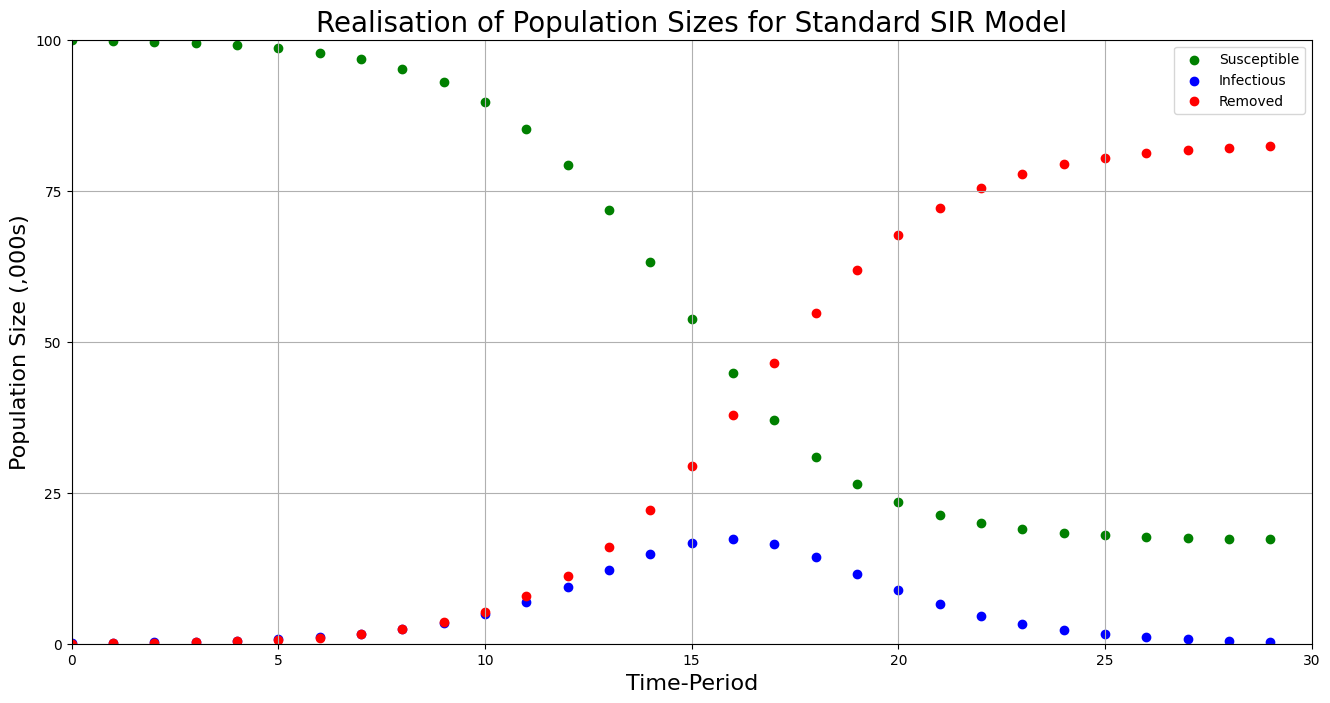
\includegraphics[width=.75\textwidth]{example_sir_model.png}
    \caption{Realisation of a standard SIR model for a population of size $N=100,000$ over 30 time-periods where $\beta=1$ and $\gamma=0.5$. ($R_0=2$)}
    \label{fig_sir_example}
  \end{figure}
\end{frame}

\begin{frame}{ABC Methods Fitting an SIR Model}
  \begin{table}
    \begin{tabular}{|l|l|}
      \hline
      \textbf{Algorithm}&\textbf{LOO-CV Score}\\
      \hline \hline
      Rejection Sampling&184,063\\\hline
      ABC-MCMC&90,713\\\hline
      ABC-SMC&19,300\\\hline
      ABC-SMC with adaptive&13,160\\perturbance \& acceptance criteria.&\\\hline
    \end{tabular}
    \caption{Leave-One-Out Cross-Validation Scores for different ABC Algorithms fitting to the SIR model in \textit{Figure \ref{fig_sir_example}}. All using identity function as the summary statistic, performing $\sim10,000$ simulations and rough tuning of acceptance rate.}
  \end{table}
\end{frame}

\begin{frame}{Adaptive ABC-SMC fitting an SIR Model}
  \begin{figure}[H]
    \centering
    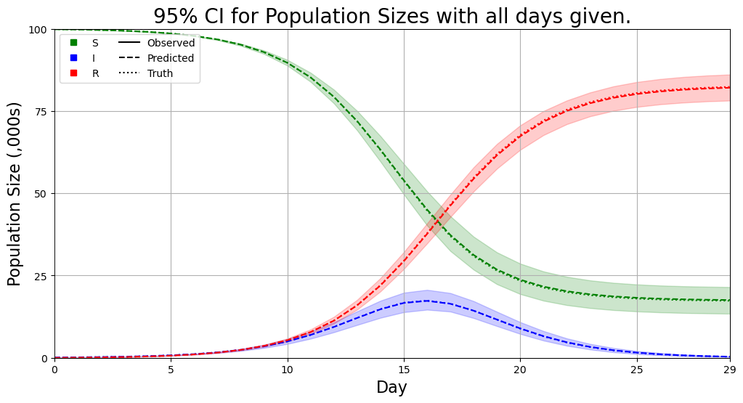
\includegraphics[width=.75\textwidth]{ABC_SMC_SIR_CI.png}
    \caption{95\% confidence interval for adaptive ABC-SMC fitting to the SIR model in \textit{Figure \ref{fig_sir_example}} using the identity function as the summary statistic. 95\% CI for $R_0$ is [1.871,2.170].}
  \end{figure}
\end{frame}

\section{Summary Statistic Methods and SIR Model}

\begin{frame}{Proposed Summary Statistics}
  These statistics were manipulated to ensure they were on a similar scale, so as to be.
  {\footnotesize\begin{multicols}{2}
    \begin{itemize}
      \item Peak size of infectious population.
      \item Date of infectious population.
      \item Final Size of susceptible population.
      \item Final Size of infectious population.
      \item Final Size of removed population.
      \item Mean Size of susceptible population.
      \item Mean Size of infectious population.
      \item Mean Size of removed population.
      \item Maximum number of infections in a day.
      \item Maximum number of removals in a day.
      \item Net Weekly changes in susceptible population ($d=4$).
      \item Net Weekly changes in infectious population.
      \item Net Weekly changes in removed population.
      \item Populations sizes on days 1,...,30 (as different statistics).
      \item Uniform random value in [12,20]
      \item $s(x)=16$.
    \end{itemize}
  \end{multicols}}
  The random and constant statistics were never chosen by any algorithm.
\end{frame}

\begin{frame}{Performance}
  \begin{table}
    \begin{tabular}{|l|l|l|}
      \hline
      \textbf{Algorithm}&\textbf{Statistics}&\textbf{ABC-SMC MSE}\\
      \hline \hline
      Control&Identity Function&121,777\\\hline
      Joyce-Marjoram&[Final Susceptible Population]&101,730,336\\\hline
      Minimum Entropy&[Mean Infectious Population,&\\
      &Mean Removed Population]&1,131,712\\\hline
      2-Step ME&[Peak Infectious Population Size,&\\
      &Mean Infectious Population,&\\
      &Mean Removed Population]&228,150\\\hline
      Semi-Automatic ABC&N/A&643,255\\\hline
    \end{tabular}
    \caption{Mean Square Error when using Adaptive ABC-SMC with the recommended summary statistics from each algorithm}
  \end{table}
\end{frame}

\begin{frame}{Visual Comparison}
  \begin{figure}[!htb]
    \centering
    \begin{minipage}{.5\textwidth}
        \centering
        \centering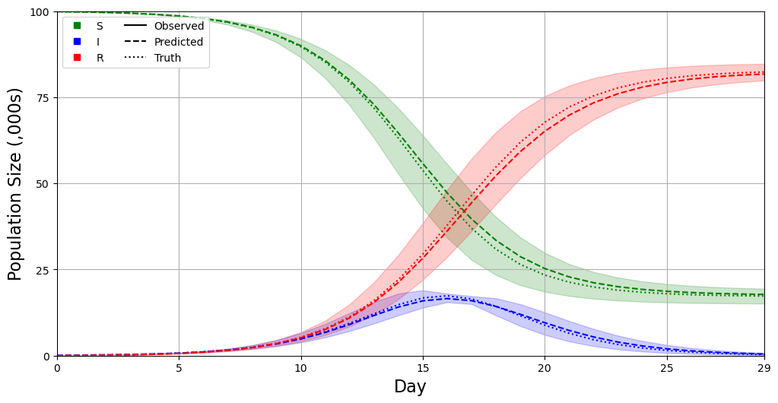
\includegraphics[width=1\textwidth]{two_step_ME_ABC_SMC_full_data_CI.png}
        \caption{95\% CI when using summary statistics chosen by Two-Step Minimum Entropy and adaptive ABC-SMC. 95\% CI for $R_0$ is [1.944,2.073].}
    \end{minipage}%
    \begin{minipage}{.5\textwidth}
        \centering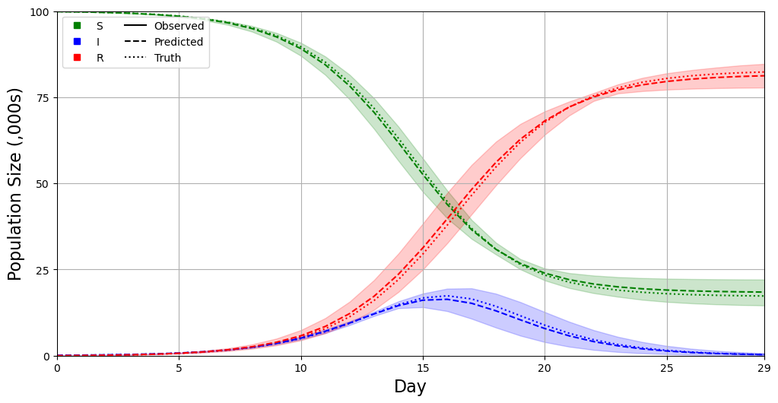
\includegraphics[width=1\textwidth]{Semi_Auto_ABC_SMC_full_data_CI.png}
        \caption{95\% CI when using summary statistics generated by semi-automatic ABC and adaptive ABC-SMC. 95\% CI for $R_0$ is [1.847,2.127].}
    \end{minipage}
  \end{figure}
\end{frame}

\begin{frame}{Projection}
  \begin{figure}[!htb]
    \centering
    \begin{minipage}{.5\textwidth}
        \centering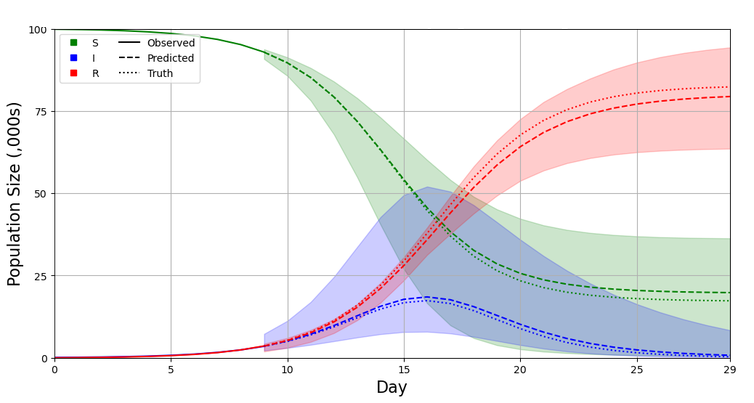
\includegraphics[width=1\textwidth]{Semi_Auto_ABC_SMC_10_days_CI.png}
        \caption{95\% CI when using summary statistics generated by semi-automatic ABC and adaptive ABC-SMC but with only the first 10 days of data. 95\% CI for $R_0$ is [1.544,3.071].}
    \end{minipage}%
    \begin{minipage}{.5\textwidth}
        \centering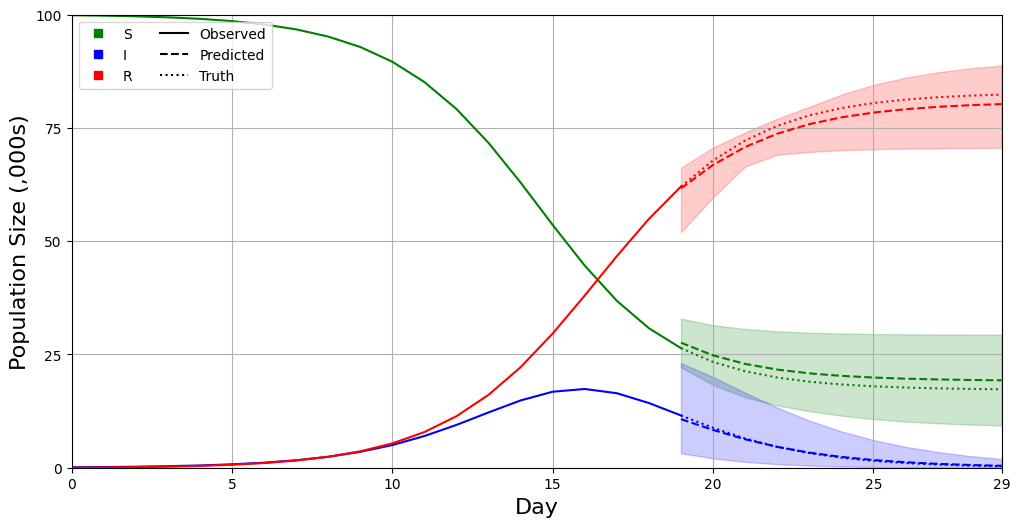
\includegraphics[width=1\textwidth]{Semi_Auto_ABC_SMC_20_days_CI.png}
        \caption{95\% CI when using summary statistics generated by semi-automatic ABC and adaptive ABC-SMC but with only the first 20 days of data. 95\% CI for $R_0$ is [1.582,2.407].}
    \end{minipage}
  \end{figure}
\end{frame}

\begin{frame}[leftcolor=CoolGrey,rightcolor=UniversityRed,div=0.85\paperwidth]{Summary}
  Yes, there are effective methods which automate the process of choosing summary statistics.
\end{frame}

\end{document}
